% ------------------------------------------------------------------------ %
% !TEX encoding = UTF-8 Unicode
% !TEX TS-program = pdflatex
% !TEX root = ../Tesi.tex
% !TEX spellcheck = it-IT
% ------------------------------------------------------------------------ %
%
% ------------------------------------------------------------------------ %
% 	INTRODUZIONE
% ------------------------------------------------------------------------ %
%
\cleardoublepage
%
\phantomsection
%
\addcontentsline{toc}{chapter}{Introduzione}
%
\chapter*{Introduzione}
%
\markboth{Introduzione}{Introduzione}	% headings
%
\label{cap:introduzione}
%
% ------------------------------------------------------------------------ %
%
Due esempi di pantografi in presa sono mostrati in figura~\ref{fig:pantoinpresa}; l'architettura asimmetrica del quadro (\ref{fig:pantoinpresa-asimm}) è quella tradizionalmente adottata per i pantografi impiegati nell'alta velocità ferroviaria.
%
% FIGURE
% ------------------------------------------------------------------------ %
% pantoinpresa
% ------------------------------------------------------------------------ %
%
\begin{figure}
%
\centering
%
\subfloat[][Architettura simmetrica\label{fig:pantoinpresa-simm}]
   {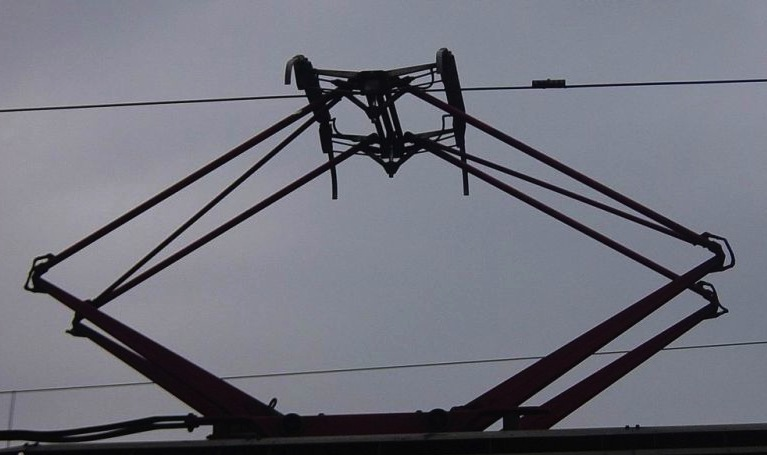
\includegraphics[width=.48\textwidth]{pantosimm}}\quad
%
\subfloat[][Architettura asimmetrica\label{fig:pantoinpresa-asimm}]
   {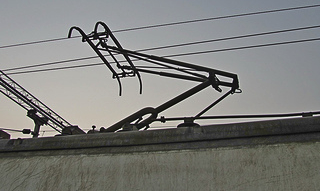
\includegraphics[width=.48\textwidth]{pantoinpresa2}}
%
\caption{Esempi di pantografi.}
%
\label{fig:pantoinpresa}
%
\end{figure}
%
% ------------------------------------------------------------------------ %
%
\subsubsection{Argomento da Approfondire1}
%
Qualche citazione \parencite{collina:2002:numerical-simulation-of-pantograph-overhead,comini:2008:fondamenti-di-termofluidodinamica-computazionale}.
%
\lipsum[1-3]
%

\bigskip

E adesso una nota a piè di pagina.\footnote{Nota a piè di pagina.}
In figura~\vref{fig:noimage} non è riportata alcuna immagine\dots o forse si?
%
% FIGURE
% ------------------------------------------------------------------------ %
% noimage
% ------------------------------------------------------------------------ %
%
\begin{figure}
%
\centering
%

\includegraphics[width=.6\textwidth]{noimage}
%
\caption{Nessuna immagine\dots Sorry.}
%
\label{fig:noimage}
%
\end{figure}
%
% ------------------------------------------------------------------------ %
%
\subsubsection{Scopi della Tesi}
%
\lipsum[1-3]
%
% ------------------------------------------------------------------------ %
%
\clearpage
%
\subsection*{Outline}
%
\par Il testo della tesi è così strutturato:
%
% ------------------------------------------------------------------------ %
%
\begin{description}
%
\item[{\hyperref[cap:statoarte]{Nel primo capitolo}}] è delineato lo stato dell'arte \lipsum[1]
%
\item[{\hyperref[cap:provesperimentali]{Il secondo capitolo}}] presenta i risultati della campagna di prove sperimentali \lipsum[2]
%
\item[{\hyperref[cap:analisinumeriche]{Nel terzo capitolo}}] si descrivono le scelte di modellazione \lipsum[3]
%
\end{description}
%
% ------------------------------------------------------------------------ %